\documentclass{standalone}
\usepackage{lmodern}
\usepackage{xcolor}
\usepackage{tikz}

\usetikzlibrary{patterns}
\renewcommand{\familydefault}{\sfdefault}

\begin{document}
    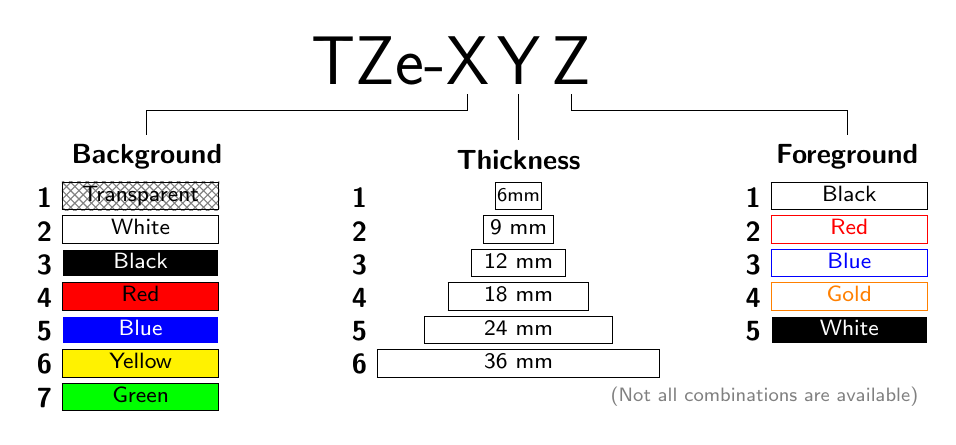
\begin{tikzpicture}
        \def\smallfont{\footnotesize\strut}
        \def\yspacing{-.425}
        \def\yoffset{-1.53}
        \def\xoffset{-4.8}
        \setlength{\fboxsep}{0pt}
        
        \tikzset{label/.style={
           anchor=north,
           align=center,
           minimum height=1em,
           inner sep=0pt
        }}

        % Title
        \node[anchor=east,font=\Huge] (X) at (-0.8,0) {TZe-};
        \node[anchor=east,font=\Huge] (X) at (-0.25,0) {X};
        \node[font=\Huge] (Y) at (0,0) {Y};
        \node[anchor=west,font=\Huge] (Z) at (0.3,0) {Z};

        % X
        \node[anchor=south west,align=left,font=\bfseries] (Xtext) at (-5.8,-1.5) {Background};
        \node[anchor=north east,align=left,font=\bfseries] at (-5.8,-1.5) {1\\ 2\\ 3\\ 4\\ 5\\6\\7};
        
     \node[label, pattern=crosshatch, pattern color=gray] 
          at (\xoffset, \yoffset + 0 * \yspacing) {\framebox[20mm][c]{\smallfont Transparent}};

    \node[label, fill=white] 
          at (\xoffset, \yoffset + 1 * \yspacing) {\framebox[20mm][c]{\smallfont White}};

    \node[label, fill=black, text=white] 
          at (\xoffset, \yoffset + 2 * \yspacing) {\framebox[20mm][c]{\smallfont Black}};

    \node[label, fill=red] 
          at (\xoffset, \yoffset + 3 * \yspacing) {\framebox[20mm][c]{\smallfont Red}};

    \node[label, fill=blue, text=white] 
          at (\xoffset, \yoffset + 4 * \yspacing) {\framebox[20mm][c]{\smallfont Blue}};

    \node[label, fill=yellow] 
          at (\xoffset, \yoffset + 5 * \yspacing) {\framebox[20mm][c]{\smallfont Yellow}};

    \node[label, fill=green] 
          at (\xoffset, \yoffset + 6 * \yspacing) {\framebox[20mm][c]{\smallfont Green}};

        % Y
        \node[anchor=south,align=left,font=\bfseries] (Ytext) at (0,-1.5) {Thickness};
        \node[anchor=north east,align=right,font=\bfseries] at (-1.8,-1.5) {1\\ 2\\ 3\\ 4\\ 5\\6}; 
        
        \def\xoffset{0}
         
        % Draw each box at a different y-coordinate with the specified width
        \node[label] at (\xoffset, \yoffset + 0 * \yspacing) {\framebox[6mm][c]{\smallfont \scriptsize 6mm}};
        \node[label] at (\xoffset, \yoffset + 1 * \yspacing) {\framebox[9mm][c]{\smallfont 9 mm}};
        \node[label] at (\xoffset, \yoffset + 2 * \yspacing) {\framebox[12mm][c]{\smallfont 12 mm}};
        \node[label] at (\xoffset, \yoffset + 3 * \yspacing) {\framebox[18mm][c]{\smallfont 18 mm}};
        \node[label] at (\xoffset, \yoffset + 4 * \yspacing) {\framebox[24mm][c]{\smallfont 24 mm}};
        \node[label] at (\xoffset, \yoffset + 5 * \yspacing) {\framebox[36mm][c]{\smallfont 36 mm}};

        % Z
        \def\xoffset{4.2}
        \node[anchor=south east,align=left,font=\bfseries] (Ztext) at (5.2,-1.5) {Foreground};
        \node[anchor=north east,align=right,font=\bfseries] at (3.2,-1.5) {1\\ 2\\ 3\\ 4\\5};
        
         \node[label, fill=white, text=black] 
              at (\xoffset, \yoffset + 0 * \yspacing) {\framebox[20mm][c]{\smallfont Black}};
        
        \node[label, fill=white, text=red] 
              at (\xoffset, \yoffset + 1 * \yspacing) {\framebox[20mm][c]{\smallfont Red}};
        
        \node[label, fill=white, text=blue] 
              at (\xoffset, \yoffset + 2 * \yspacing) {\framebox[20mm][c]{\smallfont Blue}};
        
        \node[label, fill=white, text=orange] 
              at (\xoffset, \yoffset + 3 * \yspacing) {\framebox[20mm][c]{\smallfont Gold}};
        
        \node[label, fill=black, text=white] 
              at (\xoffset, \yoffset + 4 * \yspacing) {\framebox[20mm][c]{\smallfont White}};
        

        % Lines
        \draw (X.south) -- ++ (0,-0.2) -| (Xtext.north);
        \draw (Y.south) -- ++ (0,-0.2) -| (Ytext.north);
        \draw (Z.south) -- ++ (0,-0.2) -| (Ztext.north);
        
        \node[anchor=south east, align=right, font=\scriptsize\color{gray}] at (current bounding box.south east) {(Not all combinations are available)};
    \end{tikzpicture}
\end{document}
